\documentclass[tikz,border=5mm]{standalone}
\usepackage{xcolor}
\usetikzlibrary{matrix}

\begin{document}
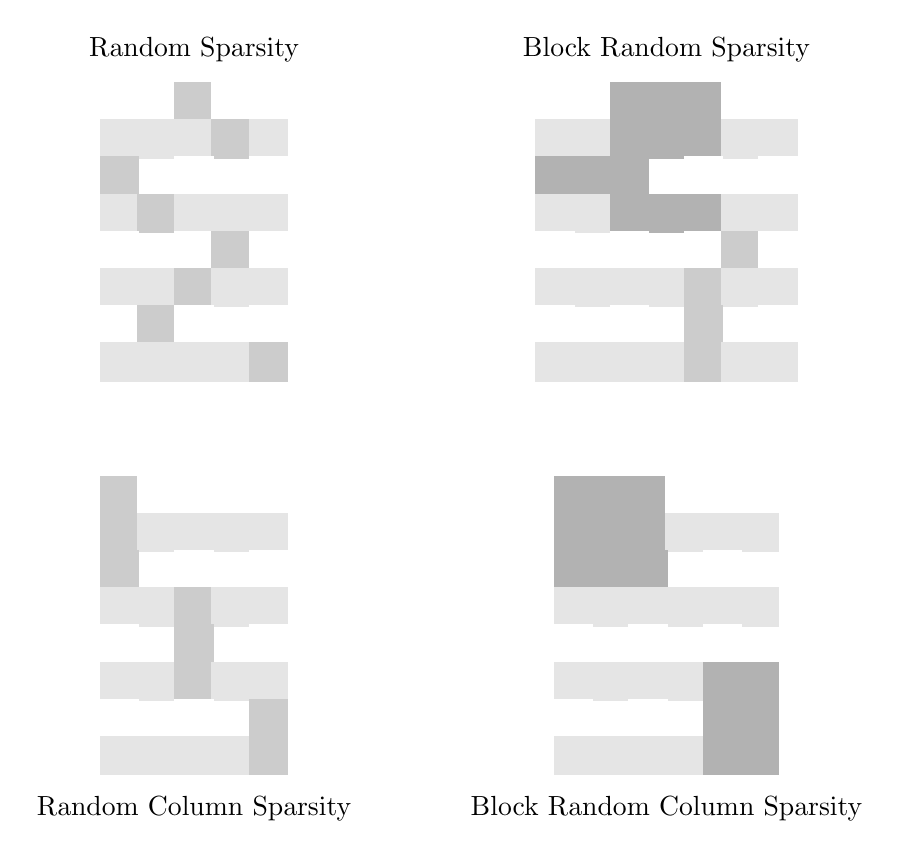
\begin{tikzpicture}[thick]
    \tikzset{
        table/.style={
            matrix of nodes,
            nodes in empty cells,
            row sep=-\pgflinewidth,
            column sep=-\pgflinewidth,
            nodes={minimum size=5mm, anchor=center},
            every even row/.style={
                nodes={fill=gray!20}
            },
            every odd column/.style={
                nodes={fill=white}
            },
            row 1/.style={
                nodes={fill=white}
            }
        },
        nonzero cell/.style={
            fill=gray!40
        },
        block nonzero cell/.style={
            fill=gray!60
        }
    }

    % Random Sparsity
    \matrix[table, label={[align=center]above:{Random Sparsity}}] (rand_sparsity) at (0,0) {
        & & |[nonzero cell]| & & \\
        & & & |[nonzero cell]| & \\
        |[nonzero cell]| & & & & \\
        & |[nonzero cell]| & & & \\
        & & & |[nonzero cell]| & \\
        & & |[nonzero cell]| & & \\
        & |[nonzero cell]| & & & \\
        & & & & |[nonzero cell]| \\
    };

    % Block Random Sparsity
    \matrix[table, label={[align=center]above:{Block Random Sparsity}}] (block_rand_sparsity) at (6,0) {
        & & |[block nonzero cell]| & |[block nonzero cell]| & |[block nonzero cell]| & & \\
        & & |[block nonzero cell]| & |[block nonzero cell]| & |[block nonzero cell]| & & \\
        |[block nonzero cell]| & |[block nonzero cell]| & |[block nonzero cell]| & & & & \\
        & & |[block nonzero cell]| & |[block nonzero cell]| & |[block nonzero cell]| & & \\
        & & & & & |[nonzero cell]| & \\
        & & & & |[nonzero cell]| & & \\
        & & & & |[nonzero cell]| & & \\
        & & & & |[nonzero cell]| & & \\
    };

    % Random Column Sparsity
    \matrix[table, label={[align=center]below:{Random Column Sparsity}}] (rand_col_sparsity) at (0,-5) {
        |[nonzero cell]| & & & & \\
        |[nonzero cell]| & & & & \\
        |[nonzero cell]| & & & & \\
        & & |[nonzero cell]| & & \\
        & & |[nonzero cell]| & & \\
        & & |[nonzero cell]| & & \\
        & & & & |[nonzero cell]| \\
        & & & & |[nonzero cell]| \\
    };

    % Block Random Column Sparsity
    \matrix[table, label={[align=center]below:{Block Random Column Sparsity}}] (block_rand_col_sparsity) at (6,-5) {
        |[block nonzero cell]| & |[block nonzero cell]| & |[block nonzero cell]| & & & \\
        |[block nonzero cell]| & |[block nonzero cell]| & |[block nonzero cell]| & & & \\
        |[block nonzero cell]| & |[block nonzero cell]| & |[block nonzero cell]| & & & \\
        & & & & & \\
        & & & & & \\
        & & & & |[block nonzero cell]| & |[block nonzero cell]| \\
        & & & & |[block nonzero cell]| & |[block nonzero cell]| \\
        & & & & |[block nonzero cell]| & |[block nonzero cell]| \\
    };
\end{tikzpicture}
\end{document}